% answers.tex —— 2005 年·普通高等学校招生考试·浙江卷·文科 · 参考答案与详细解析片段
% 由 tools/generate_projects.py 依来源总账自 2005/2005_数学真题_浙江文科_试题.md + 2005/2005_数学真题_浙江文科_解析正文.md + 2005/2005_数学真题_浙江文科_答案要点.md 生成，勿手改（改源 MD 后重跑）

\textbf{说明}：本卷答案由编者依固定题面独立推导，非官方答案；官方评分标准未经核对。

\begin{answer}
\gksolhead{1}{}

\textbf{题目}：

函数 $y = \sin\left(2x + \dfrac{\pi}{6}\right)$ 的最小正周期是\mbox{（　　）}

\begin{gkopts}(4)
\task A．$\dfrac{\pi}{2}$
\task B．$\pi$
\task C．$2\pi$
\task D．$4\pi$
\end{gkopts}

\Needspace{4\baselineskip}
\textbf{解析}

$y = \sin\left(2x + \dfrac{\pi}{6}\right)$ 的最小正周期为 $T = \dfrac{2\pi}{2} = \pi$。

\gkanswer{答案：B。}

\end{answer}
\begin{answer}
\gksolhead{2}{}

\textbf{题目}：

设全集 $U = \{1, 2, 3, 4, 5, 6, 7\}$，$P = \{1, 2, 3, 4, 5\}$，$Q = \{3, 4, 5, 6, 7\}$，则 $P \cap (\complement_U Q) =$\mbox{（　　）}

\begin{gkopts}(2)
\task A．$\{1, 2\}$
\task B．$\{3, 4, 5\}$
\task C．$\{1, 2, 6, 7\}$
\task D．$\{1, 2, 3, 4, 5\}$
\end{gkopts}

\Needspace{4\baselineskip}
\textbf{解析}

$\complement_U Q = \{1, 2\}$，故 $P \cap (\complement_U Q) = \{1, 2\}$。

\gkanswer{答案：A。}

\end{answer}
\begin{answer}
\gksolhead{3}{}

\textbf{题目}：

点 $(1, -1)$ 到直线 $x - y + 1 = 0$ 的距离是\mbox{（　　）}

\begin{gkopts}(2)
\task A．$\dfrac{1}{2}$
\task B．$\dfrac{3}{2}$
\task C．$\dfrac{\sqrt{2}}{2}$
\task D．$\dfrac{3\sqrt{2}}{2}$
\end{gkopts}

\Needspace{4\baselineskip}
\textbf{解析}

$d = \dfrac{|1 - (-1) + 1|}{\sqrt{1 + 1}} = \dfrac{3}{\sqrt{2}} = \dfrac{3\sqrt{2}}{2}$。

\gkanswer{答案：D。}

\end{answer}
\begin{answer}
\gksolhead{4}{}

\textbf{题目}：

设 $f(x) = |x - 1| - |x|$，则 $f\left[f\left(\dfrac{1}{2}\right)\right] =$\mbox{（　　）}

\begin{gkopts}(4)
\task A．$-\dfrac{1}{2}$
\task B．$0$
\task C．$\dfrac{1}{2}$
\task D．$1$
\end{gkopts}

\Needspace{4\baselineskip}
\textbf{解析}

$f\left(\dfrac{1}{2}\right) = \left|-\dfrac{1}{2}\right| - \left|\dfrac{1}{2}\right| = 0$，故 $f\left[f\left(\dfrac{1}{2}\right)\right] = f(0) = 1 - 0 = 1$。

\gkanswer{答案：D。}

\end{answer}
\begin{answer}
\gksolhead{5}{}

\textbf{题目}：

在 $(1 - x)^5 - (1 - x)^6$ 的展开式中，含 $x^3$ 的项的系数是\mbox{（　　）}

\begin{gkopts}(4)
\task A．$-5$
\task B．$5$
\task C．$-10$
\task D．$10$
\end{gkopts}

\Needspace{4\baselineskip}
\textbf{解析}

$x^3$ 的系数为 $-\mathrm{C}_5^3 - \left(-\mathrm{C}_6^3\right) = -10 + 20 = 10$。

\gkanswer{答案：D。}

\end{answer}
\begin{answer}
\gksolhead{6}{}

\textbf{题目}：

从存放号码分别为 $1, 2, \cdots, 10$ 的卡片的盒子中，有放回地取 $100$ 次，每次取一张卡片并记下号码，统计结果如下：

\begin{center}
\begingroup\setlength{\tabcolsep}{4pt}
\begin{tabular}{lcccccccccc}
\toprule
卡片号码 & 1 & 2 & 3 & 4 & 5 & 6 & 7 & 8 & 9 & 10 \\
\midrule
取到的次数 & 13 & 8 & 5 & 7 & 6 & 13 & 18 & 10 & 11 & 9 \\
\bottomrule
\end{tabular}
\endgroup
\end{center}

则取到号码为奇数的频率是\mbox{（　　）}

\begin{gkopts}(4)
\task A．$0.53$
\task B．$0.5$
\task C．$0.47$
\task D．$0.37$
\end{gkopts}

\Needspace{4\baselineskip}
\textbf{解析}

奇数号码被取到的次数为 $13 + 5 + 6 + 18 + 11 = 53$，频率为 $0.53$。

\gkanswer{答案：A。}

\end{answer}
\begin{answer}
\gksolhead{7}{}

\textbf{题目}：

设 $\alpha$、$\beta$ 为两个不同的平面，$l$、$m$ 为两条不同的直线，且 $l \subset \alpha$，$m \subset \beta$，有如下的两个命题：① 若 $\alpha \parallel \beta$，则 $l \parallel m$；② 若 $l \perp m$，则 $\alpha \perp \beta$．那么\mbox{（　　）}

\begin{gkopts}(2)
\task A．①是真命题，②是假命题
\task B．①是假命题，②是真命题
\task C．①②都是真命题
\task D．①②都是假命题
\end{gkopts}

\Needspace{4\baselineskip}
\textbf{解析}

① 若两平面平行，则分别位于两平面内的两条直线可能平行也可能异面，故为假；② 两平面内各取一条直线垂直，并不能推出两平面垂直（例如两条直线都平行于两平面的交线），故为假。

\gkanswer{答案：D。}

\end{answer}
\begin{answer}
\gksolhead{8}{}

\textbf{题目}：

已知向量 $\vec{a} = (x - 5, 3)$，$\vec{b} = (2, x)$，且 $\vec{a} \perp \vec{b}$，则由 $x$ 的值构成的集合是\mbox{（　　）}

\begin{gkopts}(4)
\task A．$\{2, 3\}$
\task B．$\{-1, 6\}$
\task C．$\{2\}$
\task D．$\{6\}$
\end{gkopts}

\Needspace{4\baselineskip}
\textbf{解析}

$\vec{a}\cdot\vec{b} = 2(x - 5) + 3x = 5x - 10 = 0$，得 $x = 2$，故集合为 $\{2\}$。

\gkanswer{答案：C。}

\end{answer}
\begin{answer}
\gksolhead{9}{}

\textbf{题目}：

函数 $y = ax^2 + 1$ 的图象与直线 $y = x$ 相切，则 $a =$\mbox{（　　）}

\begin{gkopts}(4)
\task A．$\dfrac{1}{8}$
\task B．$\dfrac{1}{4}$
\task C．$\dfrac{1}{2}$
\task D．$1$
\end{gkopts}

\Needspace{4\baselineskip}
\textbf{解析}

由 $ax^2 + 1 = x$ 得 $ax^2 - x + 1 = 0$，相切即判别式为零：$1 - 4a = 0$，故 $a = \dfrac{1}{4}$。

\gkanswer{答案：B。}

\end{answer}
\begin{answer}
\gksolhead{10}{}

\textbf{题目}：

设集合 $A = \{(x, y) \mid x, y, 1 - x - y \text{ \text{是三角形的三边长}}\}$，则 $A$ 所表示的平面区域（不含边界的阴影部分）是\mbox{（　　）}
\nopagebreak[4]
\begin{center}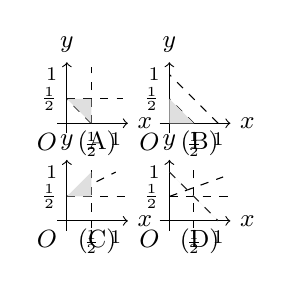
\begin{tikzpicture}[scale=0.62]
  % (A)
  \begin{scope}
    \draw[->] (-0.2,0) -- (1.25,0) node[right] {\small $x$};
    \draw[->] (0,-0.2) -- (0,1.25) node[above] {\small $y$};
    \node[below left] at (0,0) {\small $O$};
    \draw[dashed] (0.5,0) -- (0.5,1.15);
    \draw[dashed] (0,0.5) -- (1.15,0.5);
    \draw[dashed] (0.5,0) -- (0,0.5);
    \fill[gray!25] (0,0.5) -- (0.5,0.5) -- (0.5,0);
    \node at (0.62,-0.42) {\small (A)};
    \node[below] at (0.5,0) {\scriptsize $\frac{1}{2}$};
    \node[left] at (0,0.5) {\scriptsize $\frac{1}{2}$};
    \node[below] at (1,0) {\scriptsize $1$};
    \node[left] at (0,1) {\scriptsize $1$};
  \end{scope}
  % (B)
  \begin{scope}[xshift=2.1cm]
    \draw[->] (-0.2,0) -- (1.25,0) node[right] {\small $x$};
    \draw[->] (0,-0.2) -- (0,1.25) node[above] {\small $y$};
    \node[below left] at (0,0) {\small $O$};
    \draw[dashed] (0.5,0) -- (0,0.5);
    \draw[dashed] (1.0,0) -- (0,1.0);
    \fill[gray!25] (0,0) -- (0.5,0) -- (0,0.5);
    \node at (0.62,-0.42) {\small (B)};
    \node[below] at (0.5,0) {\scriptsize $\frac{1}{2}$};
    \node[left] at (0,0.5) {\scriptsize $\frac{1}{2}$};
    \node[below] at (1,0) {\scriptsize $1$};
    \node[left] at (0,1) {\scriptsize $1$};
  \end{scope}
  % (C)
  \begin{scope}[yshift=-2.0cm]
    \draw[->] (-0.2,0) -- (1.25,0) node[right] {\small $x$};
    \draw[->] (0,-0.2) -- (0,1.25) node[above] {\small $y$};
    \node[below left] at (0,0) {\small $O$};
    \draw[dashed] (0.5,-0.15) -- (0.5,1.2);
    \draw[dashed] (0,0.5) -- (1.2,0.5);
    \draw[dashed] (0,0.5) -- (1.0,1.0);
    \draw[dashed] (0.5,0) -- (1.0,0.0);
    \fill[gray!25] (0,0.5) -- (0.5,1.0) -- (0.5,0.5);
    \node at (0.62,-0.42) {\small (C)};
    \node[below] at (0.5,0) {\scriptsize $\frac{1}{2}$};
    \node[left] at (0,0.5) {\scriptsize $\frac{1}{2}$};
    \node[below] at (1,0) {\scriptsize $1$};
    \node[left] at (0,1) {\scriptsize $1$};
  \end{scope}
  % (D)
  \begin{scope}[xshift=2.1cm,yshift=-2.0cm]
    \draw[->] (-0.2,0) -- (1.25,0) node[right] {\small $x$};
    \draw[->] (0,-0.2) -- (0,1.25) node[above] {\small $y$};
    \node[below left] at (0,0) {\small $O$};
    \draw[dashed] (0.5,-0.15) -- (0.5,1.2);
    \draw[dashed] (0,0.5) -- (1.2,0.5);
    \draw[dashed] (0,1) -- (1,0);
    \draw[dashed] (0,0.5) -- (1.1,0.9);
    \fill[gray!25] (0,1) -- (1,0) -- (0.5,0.5);
    \node at (0.62,-0.42) {\small (D)};
    \node[below] at (0.5,0) {\scriptsize $\frac{1}{2}$};
    \node[left] at (0,0.5) {\scriptsize $\frac{1}{2}$};
    \node[below] at (1,0) {\scriptsize $1$};
    \node[left] at (0,1) {\scriptsize $1$};
  \end{scope}
\end{tikzpicture}
\end{center}
\nopagebreak[4]
\Needspace{4\baselineskip}
\textbf{解析}

\Needspace{5\baselineskip}
三边为正要求 $x > 0$，$y > 0$，$1 - x - y > 0$；三角形不等式给出 $x + y > 1 - x - y$、$y + (1 - x - y) > x$、$x + (1 - x - y) > y$，即
\nopagebreak[4]
\[
x + y > \frac{1}{2},\qquad x < \frac{1}{2},\qquad y < \frac{1}{2}.
\]
故区域为以 $\left(0, \dfrac{1}{2}\right)$、$\left(\dfrac{1}{2}, 0\right)$、$\left(\dfrac{1}{2}, \dfrac{1}{2}\right)$ 为顶点、不含边界的三角形。

\gkanswer{答案：A。}

\end{answer}
\begin{answer}
\gksolhead{11}{}

\textbf{题目}：

函数 $y = \dfrac{x}{x + 2}$（$x \in \mathbf{R}$，且 $x \neq -2$）的反函数是＿＿＿＿＿＿．

\Needspace{4\baselineskip}
\textbf{解析}

由 $y = \dfrac{x}{x + 2}$ 得 $yx + 2y = x$，即 $x(y - 1) = -2y$，故 $x = \dfrac{-2y}{y - 1} = \dfrac{2y}{1 - y}$。交换字母得反函数 $y = \dfrac{2x}{1 - x}$（$x \neq 1$）。

\gkanswer{答案：$y = \dfrac{2x}{1 - x}$（$x \neq 1$）。}

\end{answer}
\begin{answer}
\gksolhead{12}{}

\textbf{题目}：

设 $M$、$N$ 是直角梯形 $ABCD$ 两腰的中点，$DE \perp AB$ 于 $E$（如图）．现将 $\triangle ADE$ 沿 $DE$ 折起，使二面角 $A - DE - B$ 为 $45^\circ$，此时点 $A$ 在平面 $BCDE$ 内的射影恰为点 $B$，则 $M$、$N$ 的连线与 $AE$ 所成角的大小等于＿＿＿＿＿＿．
\nopagebreak[4]
\begin{center}\begin{tikzpicture}[scale=0.8]
  \coordinate (A) at (0,0);
  \coordinate (E) at (2.2,0);
  \coordinate (B) at (3.2,0);
  \coordinate (D) at (2.2,1.6);
  \coordinate (C) at (4.0,1.6);
  \draw (A) -- (B);
  \draw (D) -- (C);
  \draw (A) -- (D);
  \draw (B) -- (C);
  \draw[dashed] (E) -- (D);
  \draw[thick] (D) -- (E) -- (B);
  \coordinate (M) at ($(A)!0.5!(D)$);
  \coordinate (N) at ($(B)!0.5!(C)$);
  \fill (M) circle (1.2pt) node[above left] {\small $M$};
  \fill (N) circle (1.2pt) node[above right] {\small $N$};
  \node[below] at (A) {\small $A$};
  \node[below] at (E) {\small $E$};
  \node[below] at (B) {\small $B$};
  \node[above] at (D) {\small $D$};
  \node[above] at (C) {\small $C$};
\end{tikzpicture}
\end{center}
\nopagebreak[4]
\Needspace{4\baselineskip}
\textbf{解析}

折起后 $AB \perp$ 平面 $BCDE$，且由射影为 $B$ 知 $|EB| = |AE|\cos 45^\circ$，故 $|AE| = \sqrt{2}|EB|$，$\angle(EA, EB) = 45^\circ$。$M$、$N$ 是两腰中点，故 $MN$ 为梯形中位线，$MN \parallel AB$。于是 $MN$ 与 $AE$ 所成角等于 $AB$ 与 $AE$ 所成角，即 $45^\circ$。

\gkanswer{答案：$45^\circ$。}

\end{answer}
\begin{answer}
\gksolhead{13}{}

\textbf{题目}：

过双曲线 $\dfrac{x^2}{a^2} - \dfrac{y^2}{b^2} = 1$（$a > 0$，$b > 0$）的左焦点且垂直于 $x$ 轴的直线与双曲线相交于 $M$、$N$ 两点，以 $MN$ 为直径的圆恰好过双曲线的右顶点，则双曲线的离心率等于＿＿＿＿＿＿．

\Needspace{4\baselineskip}
\textbf{解析}

\Needspace{5\baselineskip}
$|MN| = \dfrac{2b^2}{a}$，以 $MN$ 为直径的圆以左焦点 $(-c, 0)$ 为心、半径 $\dfrac{b^2}{a}$。右顶点 $(a, 0)$ 在该圆上：
\nopagebreak[4]
\[
a + c = \frac{b^2}{a} = \frac{c^2 - a^2}{a},
\]
即 $a^2 + ac = c^2 - a^2$，$c^2 - ac - 2a^2 = 0$，$e^2 - e - 2 = 0$，取 $e = 2$。

\gkanswer{答案：$2$。}

\end{answer}
\begin{answer}
\gksolhead{14}{}

\textbf{题目}：

从集合 $\{P, Q, R, S\}$ 与 $\{0, 1, 2, 3, 4, 5, 6, 7, 8, 9\}$ 中各任取 $2$ 个元素排成一排（字母和数字均不能重复）．每排中字母 $Q$ 和数字 $0$ 至多只能出现一个的不同排法种数是＿＿＿＿＿＿．（用数字作答）

\Needspace{4\baselineskip}
\textbf{解析}

任取 $2$ 个字母、$2$ 个数字排列共 $\mathrm{C}_4^2\mathrm{C}_{10}^2\cdot 4! = 6 \times 45 \times 24 = 6480$ 种。同时出现 $Q$ 与 $0$ 的情形：字母含 $Q$ 的选法 $3$ 种、数字含 $0$ 的选法 $9$ 种，排列 $24$ 种，共 $3 \times 9 \times 24 = 648$ 种。故所求为 $6480 - 648 = 5832$。

\gkanswer{答案：$5832$。}

\end{answer}
\begin{answer}
\gksolhead{15}{}

\textbf{题目}：

已知函数 $f(x) = 2\sin x\cos x + \cos 2x$．

(1) 求 $f\left(\dfrac{\pi}{4}\right)$ 的值；

(2) 设 $\alpha \in (0, \pi)$，$f\left(\dfrac{\alpha}{2}\right) = \dfrac{\sqrt{2}}{2}$，求 $\sin\alpha$ 的值．

\Needspace{4\baselineskip}
\textbf{解析}

\gksubpart{(1)}

$f(x) = \sin 2x + \cos 2x$，故 $f\left(\dfrac{\pi}{4}\right) = \sin\dfrac{\pi}{2} + \cos\dfrac{\pi}{2} = 1$。

\gksubpart{(2)}

$f\left(\dfrac{\alpha}{2}\right) = \sin\alpha + \cos\alpha = \dfrac{\sqrt{2}}{2}$，即 $\sqrt{2}\sin\left(\alpha + \dfrac{\pi}{4}\right) = \dfrac{\sqrt{2}}{2}$，$\sin\left(\alpha + \dfrac{\pi}{4}\right) = \dfrac{1}{2}$。由 $\alpha \in (0, \pi)$ 得 $\alpha + \dfrac{\pi}{4} \in \left(\dfrac{\pi}{4}, \dfrac{5\pi}{4}\right)$，故 $\alpha + \dfrac{\pi}{4} = \dfrac{5\pi}{6}$，$\alpha = \dfrac{7\pi}{12}$，$\sin\alpha = \dfrac{\sqrt{6} + \sqrt{2}}{4}$。

\gkanswer{答案（1）：$1$。}

\gkanswer{答案（2）：$\dfrac{\sqrt{6} + \sqrt{2}}{4}$。}

\end{answer}
\begin{answer}
\gksolhead{16}{}

\textbf{题目}：

已知实数 $a$、$b$、$c$ 成等差数列，$a + 1$、$b + 1$、$c + 4$ 成等比数列，且 $a + b + c = 15$，求 $a$、$b$、$c$．

\Needspace{4\baselineskip}
\textbf{解析}

由等差得 $2b = a + c$，结合 $a + b + c = 15$ 得 $b = 5$，$a + c = 10$。由等比得 $(b + 1)^2 = (a + 1)(c + 4)$，即 $36 = (a + 1)(14 - a)$，整理得 $a^2 - 13a + 22 = 0$，$a = 11$ 或 $a = 2$。对应 $c = -1$ 或 $c = 8$，两组均满足等比（$12 \times 3 = 36$；$3 \times 12 = 36$）。

\gkanswer{答案：$a = 11$，$b = 5$，$c = -1$，或 $a = 2$，$b = 5$，$c = 8$。}

\end{answer}
\begin{answer}
\gksolhead{17}{}

\textbf{题目}：

袋子 $A$ 和 $B$ 中装有若干个均匀的红球和白球，从 $A$ 中摸出一个红球的概率是 $\dfrac{1}{3}$，从 $B$ 中摸出一个红球的概率为 $p$．

(1) 从 $A$ 中有放回地摸球，每次摸出一个，共摸 $5$ 次．

① 恰好有 $3$ 次摸到红球的概率；

② 第一次、第三次、第五次摸到红球的概率；

(2) 若 $A$、$B$ 两个袋子中的球数之比为 $1:2$，将 $A$、$B$ 中的球装在一起后，从中摸出一个红球的概率是 $\dfrac{2}{5}$，求 $p$ 的值．

\Needspace{4\baselineskip}
\textbf{解析}

\gksubpart{(1)}

① $P = \mathrm{C}_5^3\left(\dfrac{1}{3}\right)^3\left(\dfrac{2}{3}\right)^2 = 10 \times \dfrac{1}{27} \times \dfrac{4}{9} = \dfrac{40}{243}$。

② 指定三次均为红球、其余两次不限：$\left(\dfrac{1}{3}\right)^3 = \dfrac{1}{27}$。

\gksubpart{(2)}

\Needspace{5\baselineskip}
设 $A$ 中球数为 $n$，则 $B$ 中为 $2n$。混合后红球数为 $\dfrac{1}{3}n + 2np$，故
\nopagebreak[4]
\[
\frac{\frac{1}{3}n + 2np}{3n} = \frac{2}{5}
\Rightarrow \frac{1}{3} + 2p = \frac{6}{5}
\Rightarrow p = \frac{13}{30}.
\]

\gkanswer{答案（1）：① $\dfrac{40}{243}$；② $\dfrac{1}{27}$。}

\gkanswer{答案（2）：$p = \dfrac{13}{30}$。}

\end{answer}
\begin{answer}
\gksolhead{18}{}

\textbf{题目}：

如图，在三棱锥 $P - ABC$ 中，$AB \perp BC$，$AB = BC = \dfrac{1}{2}PA$，点 $O$、$D$ 分别是 $AC$、$PC$ 的中点，$OP \perp$ 底面 $ABC$．

(1) 求证：$OD \parallel$ 平面 $PAB$；

(2) 求直线 $PA$ 与平面 $PBC$ 所成角的大小．
\nopagebreak[4]
\begin{center}\begin{tikzpicture}[scale=0.95]
  \coordinate (P) at (0.4,2.3);
  \coordinate (A) at (-1.5,0);
  \coordinate (B) at (0.2,0.55);
  \coordinate (C) at (1.9,0);
  \coordinate (O) at ($(A)!0.5!(C)$);
  \coordinate (D) at ($(P)!0.5!(C)$);
  \draw (P) -- (A) (P) -- (B) (P) -- (C);
  \draw (A) -- (B) -- (C);
  \draw[dashed] (A) -- (C);
  \draw[dashed] (P) -- (O);
  \draw[dashed] (O) -- (D);
  \node[above] at (P) {\small $P$};
  \node[left] at (A) {\small $A$};
  \node[right] at (B) {\small $B$};
  \node[right] at (C) {\small $C$};
  \node[below] at (O) {\small $O$};
  \node[right] at (D) {\small $D$};
\end{tikzpicture}
\end{center}
\nopagebreak[4]
\Needspace{4\baselineskip}
\textbf{解析}

\gksubpart{(1)}

$O$、$D$ 分别为 $AC$、$PC$ 的中点，故 $OD \parallel PA$；又 $PA \subset$ 平面 $PAB$，$OD \not\subset$ 平面 $PAB$，故 $OD \parallel$ 平面 $PAB$。

\gksubpart{(2)}

设 $AB = BC = a$，则 $PA = 2a$。以 $B$ 为原点，$BA$、$BC$ 为 $x$、$y$ 轴建立坐标系，$A(a, 0, 0)$，$C(0, a, 0)$，$O\left(\dfrac{a}{2}, \dfrac{a}{2}, 0\right)$，设 $P\left(\dfrac{a}{2}, \dfrac{a}{2}, h\right)$。由 $|PA| = 2a$ 得 $h^2 = \dfrac{7}{2}a^2$。

\Needspace{5\baselineskip}
平面 $PBC$ 的法向量取 $\vec{n} = (h, 0, -\dfrac{a}{2})$（由 $\overrightarrow{PB} \times \overrightarrow{PC}$ 化简），$\overrightarrow{PA} = \left(\dfrac{a}{2}, -\dfrac{a}{2}, -h\right)$。设所求角为 $\theta$，则
\nopagebreak[4]
\[
\sin\theta = \frac{|\overrightarrow{PA}\cdot\vec{n}|}{|\overrightarrow{PA}||\vec{n}|} = \frac{ah}{2a\sqrt{h^2 + \frac{a^2}{4}}} = \sqrt{\frac{7}{30}}.
\]

\gkanswer{答案（1）：$O$、$D$ 为中点，故 $OD \parallel PA$，从而 $OD \parallel$ 平面 $PAB$。}

\gkanswer{答案（2）：$\arcsin\dfrac{\sqrt{210}}{30}$。}

\end{answer}
\begin{answer}
\gksolhead{19}{}

\textbf{题目}：

如图，已知椭圆的中心在坐标原点，焦点 $F_1$、$F_2$ 在 $x$ 轴上，长轴 $A_1A_2$ 的长为 $4$，左准线 $l$ 与 $x$ 轴的交点为 $M$，$|MA_1| : |A_1F_1| = 2:1$．

(1) 求椭圆的方程；

(2) 若点 $P$ 为 $l$ 上的动点，求 $\angle F_1PF_2$ 的最大值．
\nopagebreak[4]
\begin{center}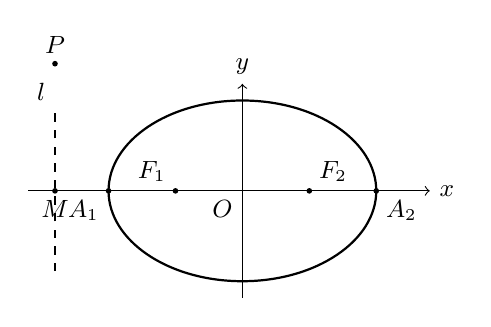
\begin{tikzpicture}[scale=0.85]
  \draw[->] (-3.2,0) -- (2.8,0) node[right] {\small $x$};
  \draw[->] (0,-1.6) -- (0,1.6) node[above] {\small $y$};
  \draw[thick] (0,0) ellipse (2 and 1.35);
  \draw[dashed] (-2.8,-1.2) -- (-2.8,1.2);
  \node[above left] at (-2.8,1.2) {\small $l$};
  \fill (-2.8,0) circle (1.2pt) node[below] {\small $M$};
  \fill (-2,0) circle (1.2pt) node[below left] {\small $A_1$};
  \fill (2,0) circle (1.2pt) node[below right] {\small $A_2$};
  \fill (-1,0) circle (1.2pt) node[above left] {\small $F_1$};
  \fill (1,0) circle (1.2pt) node[above right] {\small $F_2$};
  \node[below left] at (0,0) {\small $O$};
  \fill (-2.8,1.9) circle (1.2pt) node[above] {\small $P$};
\end{tikzpicture}
\end{center}
\nopagebreak[4]
\Needspace{4\baselineskip}
\textbf{解析}

\gksubpart{(1)}

长轴长 $4$ 得 $a = 2$，$A_1(-2, 0)$，$F_1(-c, 0)$，左准线 $x = -\dfrac{4}{c}$，故 $M\left(-\dfrac{4}{c}, 0\right)$。由 $\dfrac{|MA_1|}{|A_1F_1|} = 2$ 得 $\dfrac{4}{c} - 2 = 2(2 - c)$，即 $2c^2 - 6c + 4 = 0$，$c = 1$（$c = 2$ 退化）。故 $b^2 = 3$，椭圆为 $\dfrac{x^2}{4} + \dfrac{y^2}{3} = 1$。

\gksubpart{(2)}

\Needspace{5\baselineskip}
$l: x = -4$，设 $P(-4, t)$。记 $\theta = \angle F_1PF_2$，由两条视线斜率 $-\dfrac{t}{3}$ 与 $-\dfrac{t}{5}$ 得
\nopagebreak[4]
\[
\tan\theta = \frac{\left|-\frac{t}{3} + \frac{t}{5}\right|}{1 + \frac{t^2}{15}} = \frac{2t}{15 + t^2} \leqslant \frac{2t}{2\sqrt{15}\,t} = \frac{1}{\sqrt{15}},
\]
等号当 $t^2 = 15$ 时成立，故 $\theta_{\max} = \arcsin\dfrac{1}{4}$。

\gkanswer{答案（1）：$\dfrac{x^2}{4} + \dfrac{y^2}{3} = 1$。}

\gkanswer{答案（2）：$\arcsin\dfrac{1}{4}$。}

\end{answer}
\begin{answer}
\gksolhead{20}{}

\textbf{题目}：

已知函数 $f(x)$ 和 $g(x)$ 的图象关于原点对称，且 $f(x) = x^2 + 2x$．

(1) 求函数 $g(x)$ 的解析式；

(2) 解不等式 $g(x) \geqslant f(x) - |x - 1|$；

(3) 若 $h(x) = g(x) - \lambda f(x) + 1$ 在 $[-1, 1]$ 上是增函数，求实数 $\lambda$ 的取值范围．

\Needspace{4\baselineskip}
\textbf{解析}

\gksubpart{(1)}

图象关于原点对称即 $g(x) = -f(-x) = -x^2 + 2x$。

\gksubpart{(2)}

$-x^2 + 2x \geqslant x^2 + 2x - |x - 1|$ 即 $2x^2 \leqslant |x - 1|$。当 $x \geqslant 1$ 时 $2x^2 - x + 1 \leqslant 0$，判别式 $1 - 8 < 0$，无解；当 $x < 1$ 时 $2x^2 + x - 1 \leqslant 0$，即 $(2x - 1)(x + 1) \leqslant 0$，得 $-1 \leqslant x \leqslant \dfrac{1}{2}$。

\gksubpart{(3)}

$h(x) = -(1 + \lambda)x^2 + 2(1 - \lambda)x + 1$，$h'(x) = -2(1 + \lambda)x + 2(1 - \lambda)$ 在 $[-1, 1]$ 上恒非负。

当 $\lambda \geqslant -1$ 时 $h'$ 递减，只需 $h'(1) = -4\lambda \geqslant 0$，即 $\lambda \leqslant 0$，故 $-1 \leqslant \lambda \leqslant 0$；当 $\lambda < -1$ 时 $h'$ 递增，$h'(-1) = 4 > 0$ 恒成立。综上 $\lambda \leqslant 0$。

\gkanswer{答案（1）：$g(x) = -x^2 + 2x$。}

\gkanswer{答案（2）：$\left[-1, \dfrac{1}{2}\right]$。}

\gkanswer{答案（3）：$\lambda \leqslant 0$。}

\end{answer}